\section{Graph 3-coloring}

Remind original Knuth's algorithm at \url{http://www.iti.fh-flensburg.de/lang/algorithmen/sortieren/networks/oetsen.htm}! And prove that everything goes fine! Robusticity? %!% citovat někde

First idea: Generate all bonds with colored atoms and check the entire system (haha, complexity like $O(n^4)$ because $|E| \in O(n^2) $). Second solution: Generate a reverse-order sequence of vertices and let it order in the correct order. All pairs should meet each other, the problem to solve is whether all pairs really meet each other. After that check that the area is full like Winfree -- from one side to the other. Improvement: the check can be triggered from both sides simultaneously.

\subsection*{Set of tiles}

First of all the graph needs to have even number of vertices, thus one separated non-colored vertex has to be added if applicable. Then follow these rules which are showed in an example, see Figure \ref{fig:3-color}.
\begin{description}
	\item[Bottom line] For every pair $(2k,\,2k+1)$ there will be a bottom-type tile with non-colored numbers $(2k+2,\,2k)$ on the bottom and with all feasible\footnote{If $(2k+1,\,2k)$ are connected, same-colored numbers are omitted.} color combinations of $(2k+1,\,2k)$ on the top. From practical decoding reasons (see Winfree \cite{winfree_phd}) the sequences encoding colored numbers on the top must be physically present also wherever on the bottom DNA strand, see Figure \ref{fig:bottom_tile}. $\frac{9n}{2}$ tile types were required.
	\item[Bottom corner tiles] Both corner tiles are connected on the bottom by the highest and the lowest non-colored number, respectively, and have their special glue (\# for $-\infty$ and * for $+\infty$, respectively) on the top. These first two sets of tiles generate all colorings of given graph (without those omitted in previous step) with reverse order of numbers. $2$ tile types were required.
	\item[Inner tiles] These tiles are responsible for ordering\footnote{Principially they are the same as in Winfree \cite{winfree_phd}.}. There exist all color combinations for all different numbers with two important exceptions. There {\em do not} exist tiles with numbers of connected vertices with the same color. Thus, as soon as there appears such forbidden combination, the self assembly cannot continue and reach ``DONE''. Because the numbers are generated in reverse order they must meet each other -- note that they simply cannot ``jump'' and every number has to exchange with all the higher ones as well as with the lower ones. This implies that every forbidden combination would be revealed, thus it answers correctly if and only if the coloring is correct. The second exception are those described in the following paragraph. $9n^2$ tile types were required.
	\item[Border tiles] There are two tile types on the borders, one with sharp, one with asterisk. They keep the structure growing up.
	\item[Checking tiles] As soon as the biggest and the smallest number reach * and \#, respectively, there are two special tiles which start checking whether nothing is missing. Note that all tiles had time enough to get into correct order. In this setup checking tiles do not need to check correct order thus there can exist only two types of checking sequences ``C'' and ``D'' with all color-number combinations of middle numbers -- ``D'' with the smaller half, ``C'' with the higher half. $3n$ tile types were required.
	\item[DONE tile] If everything is checked and checking sequences meet each other, ``DONE'' tile will be connected to signalize correct solution. $1$ tile type was required.
\end{description}
\begin{figure}[H]
\begin{center}
	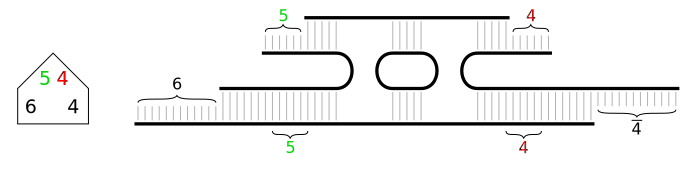
\includegraphics[scale=0.75]{./figures/3-color/bottom_tile.pdf}
	\caption{Bottom tile with desired sequences in the bottom strand.}
	\label{fig:bottom_tile}
\end{center}
\end{figure}
Summed up, this DNA algorithm requires $9n^2$ tile types. Glue complexity is ...

The first idea's binding complexity was like $O(n^4)$, the second is already $O(n^2)$, the binding complexity is $1\nicefrac{1}{2}\;n^2$. The improvement decreases it to $1\nicefrac{1}{4}\;n^2$.

\begin{figure}[H]
\begin{center}
	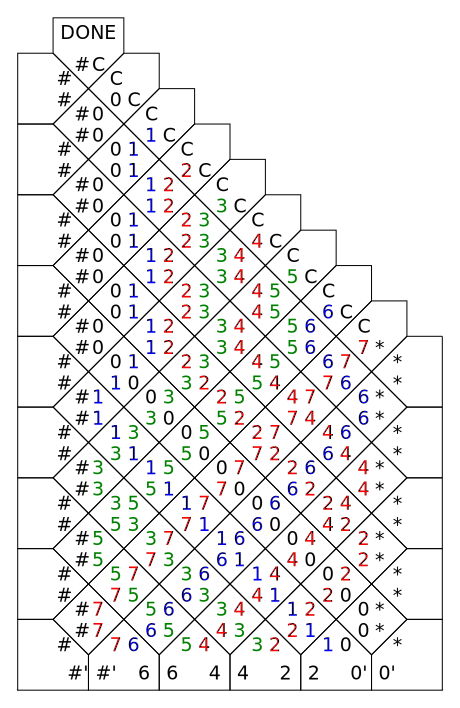
\includegraphics[scale=0.75]{./figures/3-color/3-color.pdf}
	\caption{3-color computation.}
	\label{fig:3-color}
\end{center}
\end{figure}
